\chapter{Badania eksperymentalne}
\label{results}
\section{Dane testowe}
\par{
  Przygotowanie zestawu danych testowych jasno odzwierciedlającego ograniczenie złożoności obliczeniowej rozwiązania problemu pokrycia wierzchołkowego do wielomianowej przez zastosowanie technik redukcji dziedziny do jądra problemu nie jest łatwe.
  Opisywane techniki bardzo silnie zależą od charakterystycznych cech struktury grafu, które trudno jest opisać w~prosty sposób parametrami generacji losowej.
  Dlatego też aby przygotować zestaw losowych grafów testowych przyjęto metodę generacji opartą na rozkładzie losowym stopni wierzchołków grafu w~połączeniu z~funkcją określającą współczynnik selektywności.
  Stopień każdego wierzchołka w~generowanym grafie wybierany jest losowo z~przedziału $\left<1, k\right>$ zgodnie z~rozkładem $P(k) \propto \frac{1}{k}$.
  Uzyskanie zbioru grafów losowych o~różnych parametrach owocowało bardzo niespójnymi wynikami czasów ich przetwarzania z~pomocą opisywanych w~niniejszej pracy technik, co spowodowane jest tym, że istnienie struktur redukowalnych w~grafie nie jest uzależnione wprost od liczebności wierzchołków czy też krawędzi.
  Po ,,wypróbowaniu'' kilku postaci funkcji określającej współczynnik selektywności udało się utworzyć zbiór zapewniający zbliżone do oczekiwanych pod względem przyrostu czasu przetwarzania wyniki --- przyjęta została postać $P(i, k) \propto \frac{1}{1+|i-k|}$, gdzie $i$ stanowi stopień rozpatrywanego wierzchołka.
  Następnie, w~celu uściślenia monotoniczności wyników, metodą prób i~błędów dobrano wartość parametru $k=5$.
  Dla tak wybranych parametrów wygenerowano przedstawiony w~Tabeli~\ref{tab_testdata} zbiór grafów $G=(V, E)$, mających pokrycia wierzchołkowe $C$.\\
  \begin{table}
    \begin{center}
    \caption{Wartości opisujące grafy stanowiące zbiór danych testowych.}
    \begin{tabular}{| c | c | c | c |}
      \hline
      l.p. & $|V|$ & $|E|$ & $|C|$ \\ \hline
      1 & 100 & 115 & 47 \\
      2 & 200 & 246 & 96 \\
      3 & 300 & 367 & 152 \\
      4 & 400 & 508 & 199 \\
      5 & 500 & 589 & 241 \\
      6 & 600 & 744 & 290 \\
      7 & 700 & 860 & 348 \\
      8 & 800 & 964 & 396 \\
      9 & 900 & 1113 &  445 \\
      10 & 1000 &  1218 &  501 \\ \hline
    \end{tabular} 
    \begin{tabular}{| c | c | c | c |}
      \hline
      l.p. & $|V|$ & $|E|$ & $|C|$ \\ \hline
      11 & 1100 & 1360 &  543 \\
      12 & 1200 & 1446 &  590 \\
      13 & 1300 & 1571 &  651 \\
      14 & 1400 & 1717 &  693 \\
      15 & 1500 & 1758 &  739 \\
      16 & 1600 & 2010 &  804 \\
      17 & 1700 & 2079 & 1018 \\
      18 & 1800 & 2219 & 1095 \\
      19 & 1900 & 2326 & 1119 \\
      20 & 2000 & 2463 & 1163 \\ \hline
    \end{tabular}
    \end{center}
    \label{tab_testdata}
  \end{table}
}
\section{Porównanie i~analiza szybkości działania opisanych algorytmów}
\par{
  W celu zbadania efektywności zaimplementowanych algorytmów w~redukcji czasu rozwiązania problemu pokrycia wierzchołkowego wykonano serię testów, podczas których mierzono czas wykonywania następujących operacji:

  \begin{itemize}
    \item Wyznaczenie pokrycia wierzchołkowego metodą siłową, opisaną Pseudokodem~\ref{alg_VC1} dla zestawu grafów o~pomniejszonych rozmiarach.
    \item Wyznaczenie pokrycia wierzchołkowego algorytmem własnym, opisanym pseudokodem~\ref{alg_VC2}.
    \item Wyznaczenie pokrycia wierzchołkowego algorytmem własnym po redukcji koron.
    \item Wyznaczenie pokrycia wierzchołkowego algorytmem własnym po redukcji dziedziny opartej na algorytmie przepływu w~sieci.
    \item Wyznaczenie pokrycia wierzchołkowego algorytmem własnym po wykonaniu operacji przetwarzania wstępnego i~redukcji koron.
    \item Wyznaczenie pokrycia wierzchołkowego algorytmem własnym po wykonaniu operacji przetwarzania wstępnego i~redukcji dziedziny opartej na algorytmie przepływu w~sieci.
    \item Redukcja dziedziny do jądra problemu przez usunięcie koron.
    \item Redukcja dziedziny do jądra problemu oparta na algorytmie przepływu w~sieci.
  \end{itemize}
}
\subsection{Wyznaczanie pokrycia wierzchołkowego}
\par{
  Zgodnie z~oczekiwaniami, wyznaczenie pokrycia wierzchołkowego metodą siłową, opisaną Pseudokodem~\ref{alg_VC1}, wymagało wykładniczego czasu.
  Powoduje to, że analiza grafów o~rozmiarach przedstawionych w~Tabeli~\ref{tab_testdata} trwa bardzo długo, a~wyniki pomiarów związanych z~metodą siłową zaciemniają obraz wyników pozostałych testów.
  W związku z~tym pomiar czasu działania metody siłowej został zrealizowany dla osobnego zestawu siedmiu grafów wygenerowanych opisaną metodą o~rozmiarach od dziesięciu do trzydziestu wierzchołków z~krokiem pięciu wierzchołków.
  Niestety, struktura jednego z~wygenerowanych grafów okazała się niekorzystna dla rozgałęzień algorytmu siłowego --- wyniki pomiarów czasu działania siłowej metody wyznaczania pokrycia wierzchołkowego zawiera Tabela~\ref{tab_vc_naive}.
  \begin{table}
    \begin{center}
      \caption{Czas wyznaczania pokrycia wierzchołkowego metodą siłową.}
      \begin{tabular}{| c | c | c | c |}
        \hline
        l.p. & $|V|$ & $|E|$ & czas \\ \hline
        1 & 10 & 8 & 323.884$ \mu$s \\
        2 & 15 & 20 & 9.52204 ms \\
        3 & 20 & 20 & 30.605758 ms \\
        4 & 25 & 33 & 614.454963 ms \\
        5 & 30 & 36 & 28.922161504 s \\
        6 & 35 & 35 & 1 m 27.328533967 s \\
        7 & 40 & 69 & \textit{wyłączono po 2 godzinach} \\ \hline
      \end{tabular} 
    \end{center}
    \label{tab_vc_naive}
  \end{table}
}
\subsubsection{\textbf{Czas wyznaczania pokrycia wierzchołkowego bez przetwarzania wstępnego}}\label{time_vc}
\par{
  Porównanie czasów wyznaczania pokrycia wierzchołkowego bez uprzedniego zastosowania technik przetwarzania wstępnego przedstawia Rysunek~\ref{fig_results_vc}.
  \begin{figure}
    \centering
      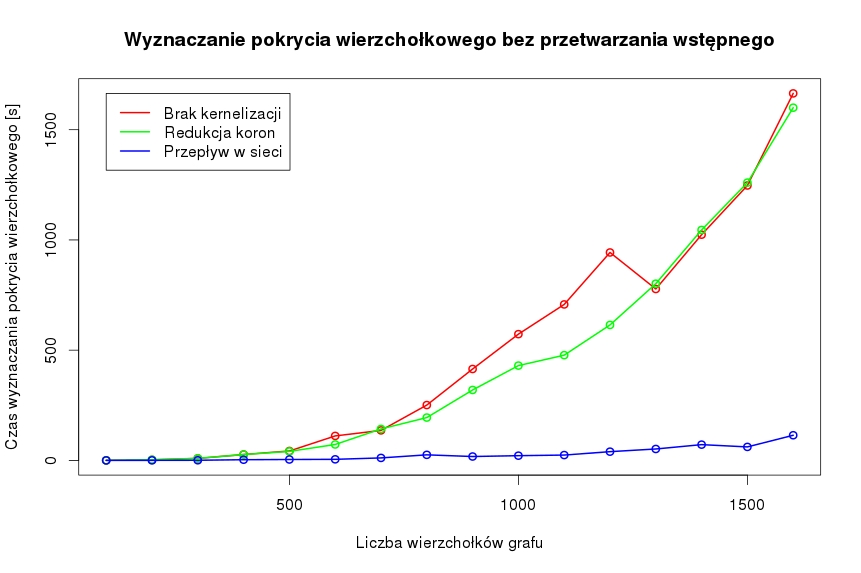
\includegraphics[width=\textwidth]{results-vc}
    \caption{Czas wyznaczania pokrycia wierzchołkowego bez przetwarzania wstępnego.}
    \label{fig_results_vc}
  \end{figure}
  Wyraźnie widoczny jest pozytywny wpływ zastosowania redukcji dziedziny do jądra problemu przez rozwiązanie przeformułowania problemu do egzemplarza problemu przepływu w~sieci.
  Za prawdopodobne uzasadnienie tego, że redukcja koron nie oferuje tak dużego przyspieszenia jak technika oparta na przepływie w~sieci uznano dwa czynniki:
  \begin{itemize}
    \item Grafy stanowiące dane testowe są ubogie w~korony.
    Wynika to z~postaci funkcji określającej współczynnik selektywności wierzchołków. Struktury koron wymagają bardzo specyficznych relacji zachodzących między zbiorami wierzchołków, mianowicie istnienia zbiorów niezależnych o~połączonym sąsiedztwie.
    W ramach procesu przygotowywania danych testowych udało się uzyskać grafy, dla których redukcja dziedziny uzyskana przez usunięcie koron była znacznie większa, jednak grafy te nie pozwalały na uzyskanie wyników dających przedstawić się w~postaci funkcji monotonicznej.
    \item Zaimplementowana technika wyznaczania koron w~grafie oparta jest na zbyt restrykcyjnym uściśleniu NT--redukcji do serii operacji działających bezpośrednio na konkretnych egzemplarzach skojarzeń.
    Najprawdopodobniej stanowi to również powód opisanych w~Podsumowaniu problemów napotkanych przy implementacji algorytmu Chena, Kanji oraz Xia.
    Pozostałe zaimplementowane egzemplarze NT--redukcji wyznaczają podzbiory różniące się od tych uzyskiwanych przez redukcję proponowaną w~pracy~\cite{KernelizationAlgorithms04}.
    Dalsze pole do badań może stanowić weryfikacja lub bardziej ogólne postacie NT--redukcji --- wykonywane za pomocą algorytmów programowania liniowego --- zapewnią lepsze rezultaty dla grafów o~strukturze zbliżonej do tych, które wykorzystano jako dane testowe.
  \end{itemize}

  Ze względu na brak optymalizacji opisywanych w~niniejszej pracy technik nie udało się wykonać pomiarów czasu wyznaczania pokrycia wierzchołkowego bez przetwarzania wstępnego dla grafów zawierających więcej niż 1600 wierzchołków.
  Pomimo nieco gorszych od oczekiwanych rezultatów należy zauważyć, że każda z~przedstawionych charakterystyk jest o~wiele rzędów wielkości lepsza niż charakterystyka uzyskana z~pomiarów czasu działania metody siłowej.
}
\subsubsection{\textbf{Czas wyznaczania pokrycia wierzchołkowego po przetwarzaniu wstępnym}}

  Porównanie czasów wyznaczania pokrycia wierzchołkowego po uprzednim zastosowaniu technik przetwarzania wstępnego przedstawia Rysunek~\ref{fig_results_vc_p}.
  \begin{figure}
    \centering
      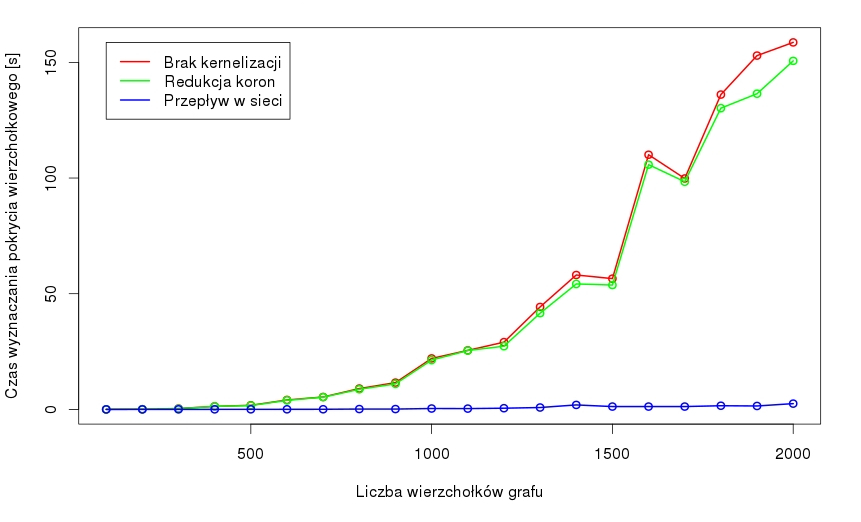
\includegraphics[width=\textwidth]{results-vc-p}
      \caption{Czas wyznaczania pokrycia wierzchołkowego po przetwarzaniu wstępnym.}
    \label{fig_results_vc_p}
  \end{figure}
  Zastosowanie prostych technik przetwarzania wstępnego opisanych w~podrozdziale~\ref{Section_preprocessing} pozwala na dodatkowe skrócenie czasu wyznaczania pokrycia wierzchołkowego w~grafach testowych o~około dwa rzędy wielkości.

  Ponieważ różnica w~czasie wyznaczania pokrycia wierzchołkowego z~zastosowaniem techniki opartej na~przepływie w~sieci między wariantem bez przetwarzania wstępnego a~wariantem z~zastosowaniem przetwarzania wstępnego jest słabo widoczna, Rysunek~\ref{fig_nf_comp} zestawia charakterystyki czasowe tych przypadków.
  \begin{figure}
    \centering
      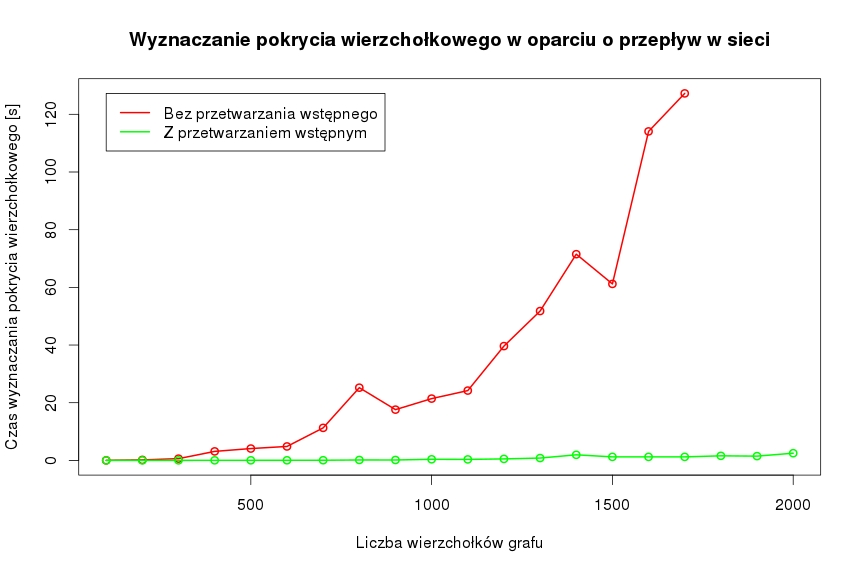
\includegraphics[width=\textwidth]{nf-comp}
    \caption{Wpływ przetwarzania wstępnego na czas wyznaczania pokrycia wierzchołkowego w~oparciu o~przepływ w~sieci.}
    \label{fig_nf_comp}
  \end{figure}

\subsection{Algorytmy przetwarzania wstępnego i~redukcji dziedziny do jądra problemu}
  Redukcja dziedziny do jądra problemu w~praktyce może mieć sens jedynie wtedy, gdy czas potrzebny wykonanie operacji zawężających przestrzeń poszukiwań pokrycia wierzchołkowego jest wielomianowy.
  W celu weryfikacji szybkości działania implementacji opisywanych technik redukcji dziedziny oraz przetwarzania wstępnego zmierzono czas potrzebny na wykonanie tych operacji dla zbioru grafów testowych. 

\subsubsection{\textbf{Algorytmy redukcji dziedziny do jądra problemu}}
  Porównanie czasów wyznaczania pokrycia wierzchołkowego bez uprzedniego zastosowania technik przetwarzania wstępnego przedstawia Rysunek~\ref{fig_results_k}.

  \begin{figure}
    \centering
      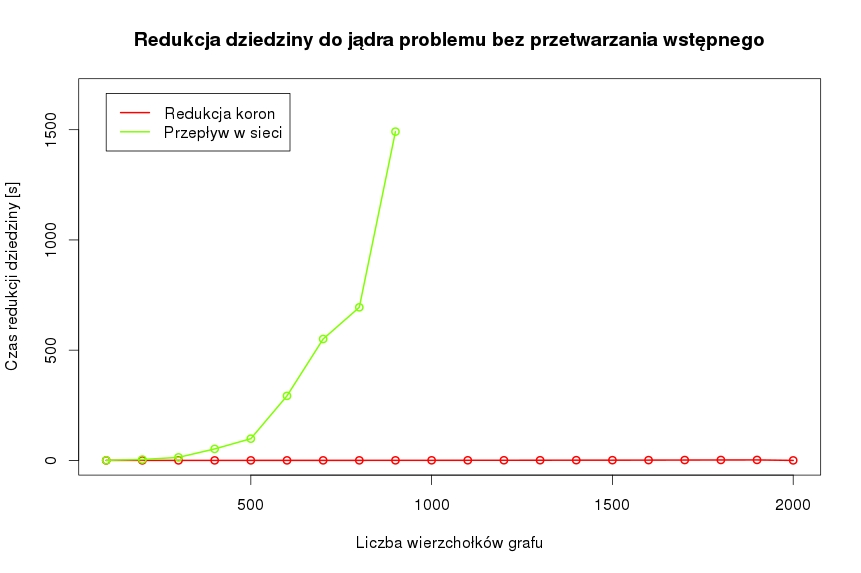
\includegraphics[width=\textwidth]{results-k}
      \caption{Czas redukcji dziedziny bez przetwarzania wstępnego.}
    \label{fig_results_k}
  \end{figure}

  Powodem niekorzystnej złożoności czasowej działania algorytmu redukcji dziedziny przez rozwiązanie przeformułowania problemu do egzemplarza problemu przepływu w~sieci jest brak optymalizacji implementacji koncepcji opisanej w~pracy~\cite{KernelizationAlgorithms04}.
  Szczegóły oraz proponowane usprawnienia opisane są w~Podsumowaniu.
  Ponieważ charakterystyka wyników pomiarów czasu działania tego algorytmu jest zdeformowana i~nie ukazuje prawdziwej jego szybkości, a~także ze względu na bardzo długi czas oczekiwania, ograniczono dziedzinę przetwarzanych przez niego grafów do zawierających najmniejszą liczbę wierzchołków.
  W związku z~zaciemnieniem na wykresie wartości wyników pomiarów czasu działania algorytmu redukcji koron, Rysunek~\ref{fig_results_k_crown} przedstawia wyłącznie tę charakterystykę.

  \begin{figure}
    \centering
      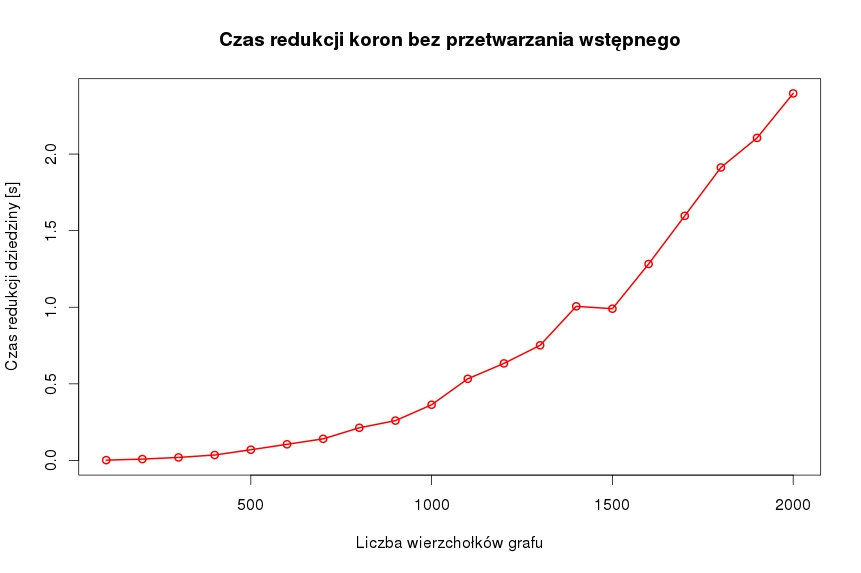
\includegraphics[width=\textwidth]{results-k-crown}
    \caption{Czas redukcji dziedziny przez wyznaczenie i~usunięcie koron bez przetwarzania wstępnego.}
    \label{fig_results_k_crown}
  \end{figure}

  Rysunek~\ref{fig_results_k_crown_p} przedstawia wpływ uprzedniego zastosowania algorytmów przetwarzania wstępnego na szybkość działania algorytmu redukcji koron.
  \begin{figure}
    \centering
      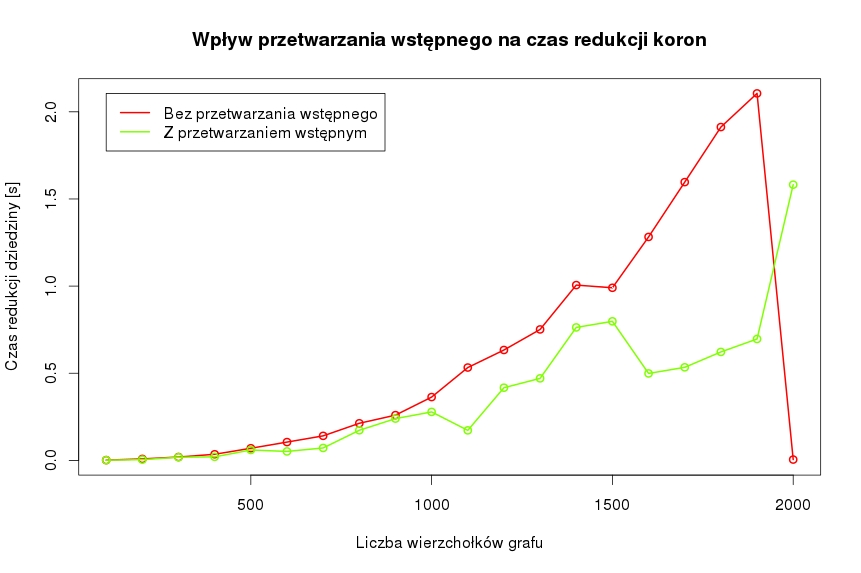
\includegraphics[width=\textwidth]{results-k-crown-p}
    \caption{Wpływ przetwarzania wstępnego na szybkość działania algorytmu redukcji koron.}
    \label{fig_results_k_crown_p}
  \end{figure}

  Zgodnie z~oczekiwaniami, zastosowanie procedur przetwarzania wstępnego przed przystąpieniem do wykonania algorytmu redukcji dziedziny do jądra problemu wpływa pozytywnie na szybkość jego działania.
  Jest to spowodowane zmniejszeniem liczby wierzchołków i~krawędzi grafu przed rozpocząciem algorytmu kernelizacji.

  Rysunek~\ref{fig_results_p} przedstawia charakterystykę czasu przetwarzania wstępnego w~zależności od liczby wierzchołków grafu.
  Pokazuje to, że operacja przetwarzania wstępnego jest wykonywana szybko nawet dla grafów o~dużej liczbie wierzchołków. Mając na uwadze przedstawione na poprzedzających wykresach korzyści płynące z~jej zastosowania nasuwa się wniosek, że warto tę operację stosować zawsze przed rozpoczęciem rozwiązywania problemu pokrycia wierzchołkowego, bez względu na zastosowane w~dalszych etapach metody redukcji dziedziny do jądra problemu oraz algorytmy wyznaczające pokrycie wierzchołkowe.
  \begin{figure}
    \label{fig_results_p}
    \centering
      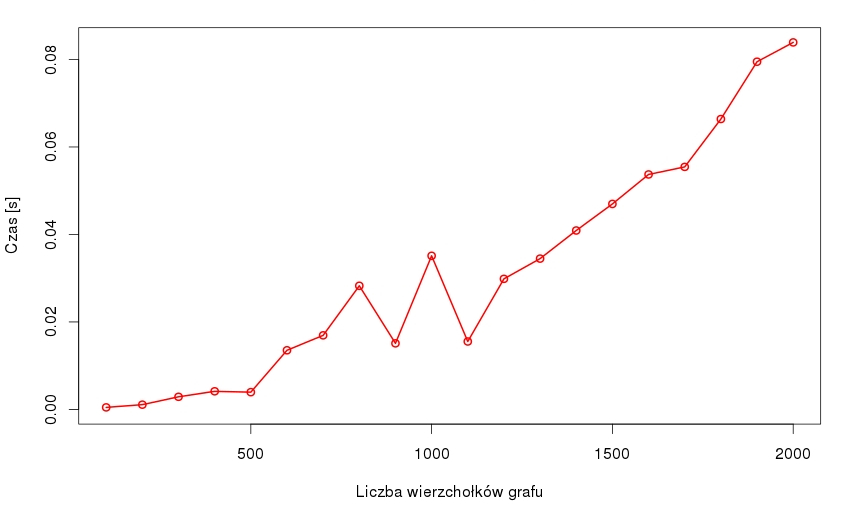
\includegraphics[width=\textwidth]{results-p}
    \caption{Czas przetwarzania wstępnego.}
  \end{figure}
\section{Środowisko testowe i~wykonywanie testów}
\par{
  W celu wykonania testów należy skopiować katalog zawarty na nośniku dołączonym do pracy, a~następnie zdefiniować zmienną środowiskową \texttt{\$GOPATH} tak, by wskazywała na ścieżkę do podkatalogu \texttt{src}.
  W następnej kolejności należy zmienić bieżącą ścieżkę na podkatalog \texttt{src/main}.
  Do wykonania pomiarów służy polecenie \texttt{go run *.go -measure N}, gdzie \texttt{N} stanowi wyrażenie regularne zawierające część nazwy przypadku testowego.
  Wyczerpująca lista zdefiniowanych przypadków testowych zawarta jest w~pliku \texttt{test-cases.go}.

  Przedstawione wyniki testów szybkości działania algorytmów uzyskano na komputerze o~nastepujących paramterach:
  \begin{itemize}
    \item Procesor Intel® Core™ i7-4800MQ (4 $\times$ 2.7 GHz)
    \item 32 GB DDR3L 1600 MHz
  \end{itemize}


  W celu realizacji testów jednostkowych należy zmienić bieżącą ścieżkę na katalog wybranego pakietu projektu i~wywołać komendę \texttt{go test}.
}
\subsection*{Generacja danych testowych}
\par{
  Istnieje możliwość wykonania testów na innych niż przedstawione w~niniejszym rozdziale danych.
  Generację grafów losowych realizuje skrypt \texttt{random-graphs.py}, umieszczony w~głównym katalogu aplikacji.
  Jest on wykonywalny z~linii poleceń.
  Wywołanie skryptu może być parametryzowane następującymi argumentami:
  \begin{itemize}
    \item \texttt{-v}, określający liczebności zbiorów wierzchołków wygenerowanych grafów.
      Wywołanie skryptu z~wartością parametru \texttt{-v 5} wygeneruje graf o~pięciu wierzchołkach, wartość \texttt{-v 5,10} spowoduje generację dwóch grafów odpowiednio o~pięciu i~dziesięciu wierzchołkach, natomiast wartość \texttt{-v 5-20,5} zaowocuje generacją czterech grafów odpowiednio o~pięciu, dziesięciu, piętnastu oraz dwudziestu wierzchołkach.
    \item \texttt{-d}, określający współczynnik selektywności wierzchołków określonego stopnia w~generowanych grafach.
      Argument ten może przyjmować identyczne postaci jak argument \texttt{-v}.
    \item \texttt{-l}, określający algorytm wizualizacji grafów. Dopuszczalne wartości opisane są w~podrozdziale~\ref{sss_internals_misc_graphviz}.
    \item \texttt{-o}, określający format obrazu wynikowego. Dopuszczalne wartości są określone formatami obsługiwanymi przez pakiet Graphviz.
  \end{itemize}

  Domyślnie skrypt generuje wyniki do katalogu \texttt{results}.
  Pliki wynikowe mają postać \texttt{V\_D.dot} oraz \texttt{V\_D.jpeg}, gdzie \texttt{V} jest wartością parametru \texttt{-v}, a~ \texttt{D} jest wartością parametru \texttt{-d} dla wygenerowanego grafu.
}
